


In today's digital landscape, utilizing various identifiers (such as usernames,
email addresses, or phone numbers) combined with passwords has become a
prevalent method for verifying an individual's identity and ensuring their
authorization to access restricted materials.

This report explores the implementation of LessPM, a passwordless password
manager that leverages WebAuthn (Web Authentication).
LessPM aims to provide an experience free from the constraints and security
implications of traditional passwords by placing a strong emphasis on
security.

LessPM is designed with a multi-layer security approach to protect
confidentiality and integrity of the user authentication process, and passwords
stored for other registered services.
By leveraging WebAuthn's asymmetric cryptographic\footnote{
  Asymmetric cryptography uses a key-pair consisting of public and private
  keys.
  The public key encrypts data, while the private key decrypts it.
  The keys are mathematically related, but deriving one from the other is
  infeasible, ensuring secure communication and data exchange.
} nature, LessPM creates a robust user authentication mechanism for sensitive
data.
This is achieved by utilizing authenticators, such as smartphones or
hardware authenticator devices, with biometric scanners to authenticate a
user through strong means.
WebAuthn, an open standard developed collaboratively by The Fast IDentity
Online Alliance (FIDO) and World Wide Web Consortium (W3C), aims to provide a
more secure authentication experience through biometric scanners on these
devices~\cite{webauthn-2}.

When a user initiates the process to register, LessPM issues a challenge
constructed by WebAuthn to the client.
The user is prompted to use a biometric scanner on their device, which then
constructs a keypair, signing this challenge, before sending this information
back to LessPM\@.
LessPM receives and stores the public key-part of the keypair for later
authentication.
This process can be seen in Figure~\ref{fig:webauthn}.

\begin{figure*}[htbp]
  \begin{center}
    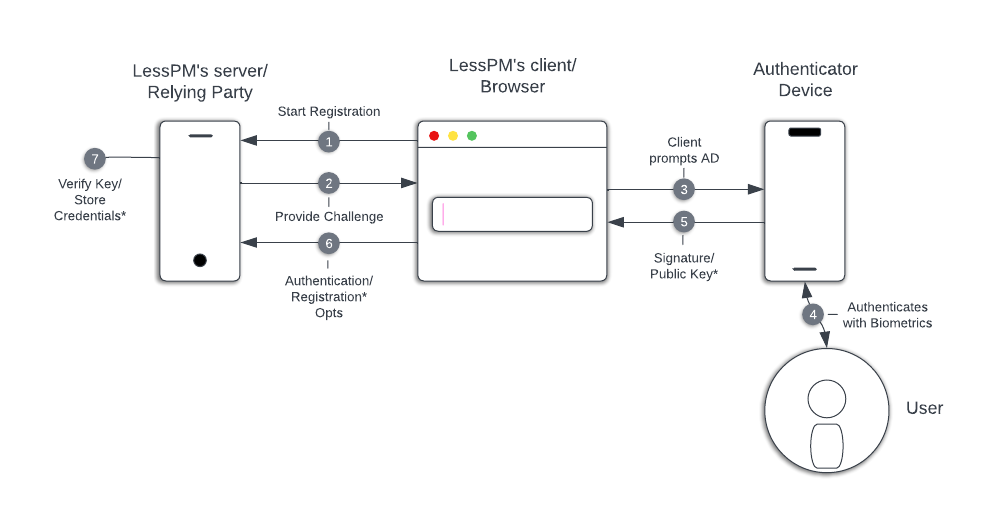
\includegraphics[scale=0.49]{images/webauthn}
    \caption{The process depicting the WebAuthn ceremonies in LessPM,
      starting with the LessPM client issuing a registration. Steps marked
      with Asterix indicate the Registration Ceremony, non-Asterix indicate
      Authentication Ceremony. }
    \label{fig:webauthn}
  \end{center}
\end{figure*}

When the user attempts to sign in, LessPM again issues a challenge,
prompting the user to use their authenticator's biometric scanner to verify
their identity and presence.
This time, however, the challenge is signed by the private key on the
authenticator device.
The device yields the signature back upon the device successfully verifying the
authenticity of the user.
LessPM then verifies this signature with the help of the public key
stored in the previous step.
This process can be seen in Figure~\ref{fig:webauthn}.

The aforementioned described processes constructs an environment such that a
malefactor is required to first access the authenticator device, and then
to bypass the device's biometric security in order to authenticate as the user
in LessPM\@.

Passwords stored in LessPM are encrypted using AES-256, a widely recognized
symmetric encryption algorithm~\cite{schneier2000secrets,rijndael_book}.
The encryption process includes using a Credential ID (CID) that is derived from
the metadata of the public key in WebAuthn, a 128-bit randomly generated salt
that is unique for each password, and a 128-bit pepper.

To maintain authentication, LessPM uses an encrypted version of JSON Web
Tokens~\cite{RFC7519} (JWT, RFC7519), inspired by JSON Web
Encryption~\cite{rfc7516} (JWE, RFC7516) which are encrypted with AES-256 as
well and attached to HTTPS requests.

The registration, authentication, and password creation/retrieval processes
all use these encrypted tokens but LessPM manages and maintains different
tokens for each step, providing an extra level of security.
Each token is valid for a limited amount of time before expiring.
An expired token prompts LessPM to deny access to unauthorized content and
forcing the user to restart the process.

LessPM's client stores the token for authentication in a cookie.
This cookie is protected by various built-in functionality in browsers, such as
the attribute \texttt{secure} to transfer the cookie over a secure connection
only, such as HTTPS\@.
Other attributes include \texttt{HttpOnly} to make sure the cookie is
inaccessible to JavaScript and Cross-Site Scripting (XSS),
\texttt{SameSite=Strict} to ensure the cookie is only sent to the same origin
it came from, and \texttt{Expires} to limit the amount the life-time of the
cookie.

LessPM uses this cookie to verify the authenticity of requests between the
client and the server.
All data the server provides to the client is dependent on the validity of
this cookie, and no information leaves the server unless it is valid.

By examining recent advancements in authentication mechanisms and the related
innovative potential of WebAuthn, we hope to illuminate the prospects of a
passwordless future in digital security.

The findings in this report is not an attempt of getting rid of trivial
concepts such as session hijacking, nor is it an empirical study of user's
perception of the technology seen.
